%%%%%%%%%%%%%%%%%%%%%%%%%%%%%%%%%%%%%%%%%%%%%%%%%%%%%%%%%%%%%%%%%%%%%%%%%%%%%%%%
\chapter{The Shortest Deposition Sequence Problem}
\label{ch:scs}
%%%%%%%%%%%%%%%%%%%%%%%%%%%%%%%%%%%%%%%%%%%%%%%%%%%%%%%%%%%%%%%%%%%%%%%%%%%%%%%%

As we have seen in Chapter \ref{ch:mlp}, the nucleotide deposition sequence
$N = N_{1} N_{2} \ldots N_{T}$ corresponding to the sequence of nucleotides
$N_i \in \{\tA, \tC, \tG, \tT\}$ added at each synthesis step during the
production of a microarray is a supersequence of all probe sequences. Ideally,
$N$ should be as short as possible in order to reduce manufacturing cost and
time. By reducing the number of synthesis steps, the chances of unintended
illumination are also reduced.

In this chapter, we study the \emph{shortest deposition sequence problem}
(SDSP), which aims at finding a shortest supersequence $N$ to synthesize a
given set of probes. The SDSP is an instance of a classical computer science
problem known as the \emph{shortest common supersequence problem} (SCSP). The
SCSP is NP-complete for strings over an alphabet of size $\sigma \geq 2$
\citep{Raiha1981}. Although several heuristics for the SCSP exist
\citep[for a survey, see][]{Fraser1995}, finding exact solutions seems to be
limited to small sets of sequences and reduced alphabet sizes. Nevertheless, we
analyze the feasibility of finding a shortest deposition sequence for a
typical microarray.

Formally, we have a set of $n$ probe sequences
$\CalP = \{p_1, p_2, \ldots p_n \}$, where each $p_k$ is drawn from an alphabet
$\Sigma$ with size $\sigma = | \Sigma |$, that is, $p_k \in \Sigma^{\ast}$ for
$1 \leq k \leq n$. For simplicity, we assume that all probe sequences
$p_k \in \CalP$ have the same length $\ell$. Our aim is to find the length $T$
of a \emph{shortest common supersequence} (SCS) $N \in \Sigma^T$ of all
$p_k \in \CalP$. The microarray production setting imposes the following
constraints to the problem: $10\,000 \leq n \leq 1\,500\,000$,
$10 \leq \ell \leq 70$, $\Sigma = \{\tA,\tC,\tG,\tT\}$,
$\sigma = | \Sigma | = 4$.

%%%%%%%%%%%%%%%%%%%%%%%%%%%%%%%%%%%%%%%%%%%%%%%%%%%%%%%%%%%%%%%%%%%%%%%%%%%%%%%%
\section{Our approach}
\label{sec:scs_ourapproach}

Several efficient algorithms for the SCSP exist, but most are based on dynamic
programming and have a $O(\ell^n)$ space complexity \citep{Itoga1981,Foulser1992},
and they can thus only be used to solve problem instances with small $n$. The
only feasible approach to compute an exact solution to the SCSP for large $n$
seems to be a branch-and-bound search because its space complexity is merely
$O(n \cdot \ell)$ for simple implementations.

\begin{figure}[t]\centering
\includegraphics[width=0.95\textwidth]{scs_tree}
\caption{\label{fig:scs_tree}%
  Complete tree $\CalT$ with height $h = 3$ representing all sequences formed
  with $0 \leq r \leq h$ letters of the alphabet $\Sigma = \{\tA,\tB,\tC\}$.
  Each node has $\sigma = | \Sigma | = 3$ children.}
\end{figure}

Consider a complete tree $\CalT$ of degree $\sigma$ with edges labeled with the
letters of the alphabet $\Sigma$. The root node represents an empty sequence,
and each node has $\sigma$ children, one for each possible letter of the
alphabet. A node $f$ of $\CalT$ represents a sequence $d_f$ formed by the
sequence of letters in the path from the root to $f$. The nodes of such a tree
with height $h$ contain all sequences formed with $0 \leq r \leq h$ letters of
$\Sigma$. Figure \ref{fig:scs_tree} shows $\CalT$ for
$\Sigma = \{\tA,\tB,\tC\}$.

The SCSP can be solved by generating all possible candidate sequences $N$ with a
length $r$ (starting with $r = \ell$), checking whether each of them is a
supersequence of all $p \in \CalP$. If no supersequence of length $r$ is
found, $r$ is increased, and all candidate sequences with the new length
are generated and examined. When a supersequence is found, the value of $r$
denotes the length of the shortest common supersequence. This corresponds to a
\textit{breadth-first} search on a tree $\CalT$ where the height $h$ is
increased until a supersequence is found. In Figure \ref{fig:scs_tree}, a
possible breadth-first traversal of $\CalT$ is to visit the nodes in the
following order: \Seq{A}, \Seq{B}, \Seq{C}, \Seq{AA}, \Seq{AB}, \Seq{AC},
\Seq{BA}, \Seq{BB}, \Seq{BC}, \Seq{CA}, \Seq{CB}, \Seq{CC}, \Seq{AAA},
\Seq{AAB}, \Seq{AAC}, \Seq{ABA}, \Seq{ABB}, \Seq{ABC}, \Seq{ACA}, $\ldots$
\Seq{CCC}. Alternatively, the nodes of $\CalT$ could be explored in a
\textit{depth-first} fashion, which searches ``deeper'' in the tree whenever
possible. In Figure \ref{fig:scs_tree}, a possible depth-first traversal of
$\CalT$ visits the nodes in the following order: \Seq{A}, \Seq{AA}, \Seq{AAA},
\Seq{AAB}, \Seq{AAC}, \Seq{AB}, \Seq{ABA}, \Seq{ABB}, \Seq{ABC}, \Seq{AC},
\Seq{ACA}, \Seq{ACB}, \Seq{ACC}, \Seq{B}, \Seq{BA}, \Seq{BAA}, $\ldots$
\Seq{CCC}.

The advantage of a depth-first search is that, when combined with a
branch-and-bound strategy, it results in an efficient way of exploring the
search space. A branch-and-bound strategy means that, before exploring a branch
of $\CalT$, we check whether it has a chance of leading to a better solution
than the best solution found so far \citep{Horowitz1996}; if it does not, the
branch is skipped. The implications of this strategy are two-fold. First, it
requires that we already have a supersequence (although it might not be the
shortest one) even before the search starts. This approximate solution is an
upper bound on the length of the SCS used to delimit the search-space that needs
to be explored; the shorter it is, the more branches of the tree are likely to
be skipped. During the search, we keep track of the best solution found and
update it whenever a shorter supersequence is encountered. Section
\ref{sec:scs_ubound} describes heuristic algorithms that can be used to produce
an approximate solution to the SCSP relatively quickly. Second, the
branch-and-bound strategy requires a way of checking whether a node can lead to
a better solution or not, i.e., we need a lower bound on the length of any
supersequence that can be found from a given node (each node in $\CalT$ is a
prefix of a set of candidate sequences). Section \ref{sec:scs_lbound}
discusses possible lower bounds for the SCSP. As we shall see, the success of the
branch-and-bound search depends on finding a good lower bound that can be
computed quickly.

In principle, a branch-and-bound strategy could also be used with a
breadth-first search. However, doing so would require keeping track of the
branches of the tree that need to be further investigated, which would consume a
prohibitive amount of memory as the search reaches deeper levels of the tree.
A depth-first search, on the other hand, does not require such bookkeeping. Each
child of a node is reached by a different letter of the alphabet, and they can
be examined in a pre-defined order, e.g., alphabetical order. When a node is
skipped because it cannot lead to a better solution, the search backtracks and
continues on the next branch in the depth-first order.

When the search is at a node $f$ of the tree, its corresponding sequence $d_f$
is a prefix of a set of candidate sequences. For each sequence
$p_k \in \CalP$, $d_f$ is a supersequence of a (possibly empty) prefix of $p_k$.
Let $c_k$ be the longest prefix of $p_k$ which is a subsequence of $d_f$, and
$\bar{c}_k$ be the remainder of $p_k$ such that $p_k$ is a
concatenation of $c_k$ and $\bar{c}_k$. In order to be a proper supersequence of
$\CalP$, $d_f$ must be extended with a suffix that is a supersequence of the set
$\CalR = \{\bar{c}_1, \bar{c}_2, \ldots \bar{c}_n\}$. The lower bounds discussed
in Section \ref{sec:scs_lbound} are used to estimate the minimum length $\CalL_f$ of
the SCS of all $\bar{c}_k \in \CalR$. Since we know the length of $d_f$, the
length of any supersequence of all $p_k \in \CalP$ that can be reached from $f$
is at least $|d_f| + \CalL_f$.

%%%%%%%%%%%%%%%%%%%%%%%%%%%%%%%%%%%%%%%%%%%%%%%%%%%%%%%%%%%%%%%%%%%%%%%%%%%%%%%%
\section{Upper bounds}
\label{sec:scs_ubound}

Two well-known heuristics are used to compute an approximate solution to the
SCSP and set an initial upper bound on the length of the SCS for our
branch-and-bound search: Alphabet-leftmost and Majority-merge
\citep[see][]{Fraser1995a,Jiang1995,Rahmann2003}.

\paragraph{Majority-merge.} The Majority-merge algorithm starts with an empty
supersequence and builds it, iteratively, by keeping track of the prefixes of
each input sequence that have already been ``consumed'' by the supersequence. At
each step, it selects the next character of the supersequence by examining the
first non-consumed characters of each input sequence and picking the most
frequent one.

\paragraph{Alphabet-leftmost.} Let $\psi$ be a permutation of the letters of
$\Sigma$. If $\ell$ is the length of the longest input sequence and $N$ is an
$\ell$-fold repetition of $\psi$, $N$ is a supersequence of the set.
Alphabet-leftmost heuristically finds a shorter supersequence by computing a
left-most embedding of each input sequence in $N$ and removing the last
``unused'' characters of $N$. According to \citet{Rahmann2003} and to our own
empirical results, this algorithm is hard to be outperformed in practice. The
choice of the permutation $\psi$ is not important, but if the alphabet is small
(as it is in our setting), it is worth trying all possible permutations of
$\Sigma$ and selecting the shortest one.

%%%%%%%%%%%%%%%%%%%%%%%%%%%%%%%%%%%%%%%%%%%%%%%%%%%%%%%%%%%%%%%%%%%%%%%%%%%%%%%%
\section{Lower bounds}
\label{sec:scs_lbound}

Perhaps the simplest lower bound on the length of the SCS is to take the length
of the longest sequence in $\CalP$. In this section we examine more interesting
(and tighter) lower bounds that can be used in our branch-and-bound search.

\paragraph{Counting occurrences of single letters.}
Let $\CalN(c)$ be the maximum number of occurrences of the letter $c$ over all
sequences $p_k \in \CalP$. Clearly, a shortest common supersequence must
have, at least, $\CalN(c)$ occurrences of each $c \in \Sigma$.

For instance, consider the set of sequences $\CalP = \{p_1, p_2, p_3 \}$ of
length $\ell = 8$, where $\Sigma = \{\tA,\tB,\tC \}$, $p_1 = \Seq{CABBABAC}$,
$p_2 = \Seq{CCABBABC}$ and $p_3 = \Seq{BBBBAACC}$. The maximum number of
occurrences of $\tA$ is $\CalN(\tA)=3$. Similarly, $\CalN(\tB)=4$ and
$\CalN(\tC)=3$. The SCS must thus contain, at least, 3 $\tA$s, 4 $\tB$s, and 3
$\tC$s, i.e., its length cannot be shorter than
$\CalN(\tA) + \CalN(\tB) + \CalN(\tC) = 10$.

\paragraph{Counting pairs and triples.}

The same idea can be extended to count occurrences of pairs of letters or even triples,
using the same reasoning as above. For instance, let
$\CalN(c_i \, c_j)$ be the maximum number of occurrences of the subsequence
$c_i \, c_j$ (i.e., the subsequence consisting of letters $c_i$ and $c_j$, in
this order) over all sequences $p_k \in \CalP$. A shortest common
supersequence must have, at least, $\CalN(c_i \, c_j)$ occurrences of each
subsequence formed with letters $c_i, c_j \in \Sigma$.

In the example above, $\CalN(\Seq{AA}) = 3$ as $p_1 = \Seq{CABBABAC}$ contains 3
distinct \Seq{AA} subsequences. Similarly, $\CalN(\Seq{AB}) = 4$,
$\CalN(\Seq{AC}) = 4$, $\CalN(\Seq{BA}) = 8$, $\CalN(\Seq{BB}) = 6$,
$\CalN(\Seq{BC}) = 8$, $\CalN(\Seq{CA}) = 4$, $\CalN(\Seq{CB}) = 6$, and
$\CalN(\Seq{CC}) = 3$. Each $p_k \in \CalP$ has length $\ell = 8$,
and can thus accommodate ${8 \choose 2} = 28$ pairs. The SCS must contain
at least
%%
\[
\sum_{c_i, c_j \in \Sigma} \CalN(c_i \, c_j) = 46
\]
distinct pairs, and its length thus cannot be shorter than 11 (a sequence of
length 10 can only contain ${10 \choose 2} = 45$ pairs).

It might seem intuitive to think that counting pairs should produce tighter
lower bounds than counting single letters (as it did in this example, giving a
lower bound of 11 instead of 10) because the former is based on ``more
information''. In practice, however, counting pairs or triples rarely produced
better results than counting single letters in our microarray production
setting. Another disadvantage of counting pairs and triples is that they require
$O(\ell^2)$ and $O(\ell^3)$ time for each $p_k \in \CalP$, respectively. In
contrast, we can count the occurrences of single letters in linear time.

\subsection{Looking for better lower bounds}

We investigated two relations on strings in an attempt to find tighter lower
bounds on the length of the SCS. The first one was the following relation, valid
for any string $w \in \Sigma^\ast$ and letters $x,y \in \Sigma$, with $x \ne y$:
%%
\[
|w|_{xy} + |w|_{yx} = |w|_{x} \times |w|_{y},
\]
%%
where $|w|_{x}$ refers to the number of occurrences of $x$ in $w$, and
$|w|_{xy}$ refers to the number of occurrences of the subsequence $xy$ in $w$.

Since this relation holds for any sequence, it should also hold for the
supersequence. We then analyzed a similar relation based on the
least number of occurrences of single letters and pairs over all sequences
$p \in \CalP$, $\CalN(x)$
and $\CalN(x \, y)$, respectively, and found that, in the majority of cases,
%%
\[
\CalN(x \, y) + \CalN(y \, x) \leq \CalN(x) \times \CalN(y).
\]
This contrasted with our initial intuition that counting pairs would ``carry
more information'' than counting single letters. If we had found that
$\CalN(x \, y) + \CalN(y \, x) > \CalN(x) \times \CalN(y)$, we could produce a
lower bound on the length of the SCS by creating several relations of this form,
and forcing an increase in the values of $\CalN(x)$ and $\CalN(y)$ for each
$x,y \in \Sigma$, until
$\CalN(x \, y) + \CalN(y \, x) = \CalN(x) \times \CalN(y)$.

Another interesting relation that seemed promising in the beginning was the
Cauchy inequality \citep{Salomaa2003,Mateescu2004}:
%%
\[
|w|_{y} \times |w|_{xyz} \leq |w|_{xy} \times |w|_{yz},
\]
%%
where the notations $|w|_{y}$, $|w|_{xy}$ and $|w|_{xyz}$ refer to the number of
occurrences of single letters, pairs and triples in $w$, respectively, for
$x, y, z \in \Sigma$ and $w \in \Sigma^\ast$.

Again, we analyzed a similar relation with respect to the minimum number of
occurrences of single letters, pairs, and triples over all sequences
$p \in \CalP$, $\CalN(x)$, $\CalN(x \, y)$ and $\CalN(x \, y \, z)$,
respectively, and found that, in all cases we examined,
%%
\[
\CalN(y) \times \CalN(x \, y \, z) \leq \CalN(x \, y) \times \CalN(y \,z).
\]

Contrary to the previous relation, there was no intuitive notion to predict how
this relation behaves in practice. Nevertheless, if we had found that, in some
cases, $\CalN(y) \times \CalN(x \, y \, z) > \CalN(x \, y) \times \CalN(y \,z)$,
we could estimate the length of the SCS by increasing the values of $\CalN(yz)$
and $\CalN(xy)$ until
$\CalN(y) \times \CalN(x \, y \, z) \leq \CalN(x \, y) \times \CalN(y \,z)$.

Since we could not use any of these two relations to compute a lower bound on
the SCS, the method of counting single letters remains, to our knowledge, the
best lower bound for our setting.

%%%%%%%%%%%%%%%%%%%%%%%%%%%%%%%%%%%%%%%%%%%%%%%%%%%%%%%%%%%%%%%%%%%%%%%%%%%%%%%%
\section{Implementation}
\label{sec:scs_implementation}

In this section, we describe in more detail an implementation of the
branch-and-bound search to solve the shortest deposition sequence problem for a
set of probe sequences $\CalP = \{p_1, p_2, \ldots p_n \}$ of a typical
microarray, where $p_k \in \Sigma^{\ell}$ for $1 \leq k \leq n$, and
$\Sigma = \{\tA,\tC,\tG,\tT\}$.

Before the search starts, both Majority-merge and Alphabet-leftmost are used to
find a supersequence $U$ and set an initial upper bound on the length of the
SCS. Since the alphabet in our problem is small ($\sigma = 4$),
Alphabet-leftmost is run with all $4! = 24$ permutations of $\Sigma$. Both
algorithms are relatively fast, and their influence on the total running time is
negligible because they are executed only once. During the search, $U$ is
updated whenever a shorter supersequence is found.

The search starts from the root node and proceeds down the tree $\CalT$ in a
depth-first fashion. At every node $f$, we first check whether the sequence
$d_f$ represented by $f$ is a supersequence of all probe sequences
$p_k \in \CalP$. If it is not, a lower bound $\CalL_f$ on the length of the shortest
supersequence having $d_f$ as a prefix is computed. The search proceeds to a
child of $f$ only if $|d_f| + \CalL_f < |U|$. Otherwise, the branch rooted at $f$ is
skipped, and the search proceeds to a non-visited sibling node of $f$. If all
sibling nodes of $f$ have already been visited, the search backtracks and
continues on the next node in the depth-first order.

Unlike the initial upper bound computation, we cannot afford to compute all
lower bounds described in Section \ref{sec:scs_lbound} to choose the best result
because this estimation is done at every node of the tree. In fact, finding a
good lower bound that can be computed quickly is the key to the success of our
search. Initial experiments revealed that the best alternative is to compute the
lower bound based on the number of occurrences of single letters, as it
produces the best results in the majority of cases (in our experiments, counting
pairs produced tighter bounds in only 10\% of the cases). Moreover, it is
significantly faster to compute and consumes less memory than the other lower
bounds.

Because of the branch-and-bound strategy, whenever another supersequence is
found, we know that it is shorter than the previously known supersequence
(otherwise the search would not reach its corresponding node). In this case, $U$
is updated and the search backtracks to a node $f$ where $|d_f| + \CalL_f < U$.

\paragraph{Visiting Order.} The sooner a shorter supersequence is found during
the search, the higher is the chance of skipping branches of $\CalT$. The order
in which the children of a node are examined is important because it may help
finding a shorter supersequence earlier rather than later. According to
\citet{Chase1976}, a supersequence that is a repeated permutation of the
alphabet maximizes the number of distinct subsequences that can be embedded in
it. Hence, using a fixed visiting order for the branch-and-bound search, e.g.,
$(\tA, \tC, \tG, \tT)$, is not a good strategy because doing so results in the
first candidate sequences having a prefix consisting of a repetition of the
same letter.

For this reason, the first children of a node to be visited, in our
implementation, depends on the last letter appended to the sequence represented
by the current node (i.e., the label of the last edge on the path to the current
node), in such a way that the first candidate sequences consist of a repeated
permutation of the alphabet. For instance, if a permutation $(\tA,\tC,\tG,\tT)$
is fixed, and the last appended letter is $\tG$, then the first child node to
be visited is the one reached with $\tT$, followed by the one reached with $\tA$
and so on.

\paragraph{Computing lower bounds.} 
In order to speed up the lower bound computation, we keep track of the length
$I_k$ of the longest prefix $c_k$ of each sequence $p_k \in \CalP$ that is a
subsequence of the $d_f$ corresponding to the current node $f$. When the search
proceeds to a child node $g$ (incrementing the sequence $d_f$ with a letter $x$
to produce $d_g$), we examine every input sequence $p_k \in \CalP$, and
increment $I_k$ if and only if $p_k[I_k + 1] = x$.

When the search proceeds from the child node back to its parent, a similar
procedure must also be executed to update each $I_k$. In order to make the
updates reversible, however, we need to know whether the last letter of $c_k$
corresponds to the letter that is being deleted from $d_g$. Therefore, when an
index $I_k$ is incremented, we set $R_k[I_k] = |d_g|$. When the search goes from
child node $g$ to parent node $f$, index $I_k$ is decremented if and only if a)
$p_k[I_k] = x$, where $x$ corresponds to the edge of the tree that is being
traversed back, and b) $R_k[I_k] = |d_g|$. Indices $I_k$ and $R_k$ require, in
total, $O(n)$ and $O(n \cdot \ell)$ space, respectively.

During the search, we also keep track of the number of occurrences of each
letter of the alphabet for each input sequence $p_k \in \CalP$, and the maximum
number of occurrences of each letter over all sequences. This requires
an extra $O(n \cdot \sigma)$ space.

Finally, we also store the lower bounds for every node in the path from the root
to the current node, so that they do not need to be re-computed when the search
backtracks. The maximum size required for these values is $O(T)$, where $T$ is
the length of the SCS. In this way, we significantly reduce the total running
time of the search at the expense of an increase in space complexity of the
branch-and-bound search from $O(n)$ to $O(n(\ell \cdot \sigma) + T)$.

%%%%%%%%%%%%%%%%%%%%%%%%%%%%%%%%%%%%%%%%%%%%%%%%%%%%%%%%%%%%%%%%%%%%%%%%%%%%%%%%
\section{Results}
\label{sec:scs_results}

Three variables determine the time required to completely traverse the search
space with our branch-and-bound algorithm: $\sigma$, $\ell$ and $n$. The size of
the alphabet, $\sigma$, determines the breadth of the tree and the number of
candidate sequences of a given length. The length $\ell$ of the probe
sequences will ultimately affect the length of the shortest common supersequence
and, as a result, the depth of the search. The number of sequences, $n$,
influences the time spent at each node computing the lower bounds.

Among them, $\sigma$ is the most critical factor as it increases the size of the
search-space exponentially (the number of nodes in level $h$ of the tree is
$\sigma^{(h - 1)}$). Empirical results showed that the smallest variation in
$\sigma$ can drastically increase total running time. In contrast, the value of
$n$ is the less critical one, since the work done at each node is nearly $O(n)$.
Fortunately, the microarray production setting constrains $\sigma$ and $\ell$
to relatively small values, although $n$ is much larger than any other known
similar study --- a branch-and-bound depth-first search was also used by
\citet{Fraser1995}, but the problem instances had $n \leq 24$.

Table \ref{tab:scs} shows the results of running our branch-and-bound search on
several problem instances. In order to evaluate the impact caused by varying
$\sigma$, $\ell$ and $n$ more quickly, in most experiments we used a smaller
alphabet ($\sigma = 3$) than required by the microarray production setting.

\begin{table}[t!]\centering
\caption{\label{tab:scs}
  Initial upper bound (IUB), length of the shortest common supersequence (SCS)
  and approximate running time (in minutes) for problem instances with varying
  alphabet sizes $\sigma$, length $\ell$ and number $n$ of probe sequences.}
\footnotesize{
\begin{tabular}{rrrrrr}
$\sigma$ & $\ell$ &       $n$ & IUB & SCS &    Time \\ \hline
       3 &     10 &  $1\,000$ &  28 &  27 &   $0.1$ \\
       3 &     10 & $10\,000$ &  29 &  28 &   $0.2$ \\ 
       3 &     15 & $10\,000$ &  40 &  39 &   $6.3$ \\
       3 &     17 &     $100$ &  40 &  39 &  $34.3$ \\
       3 &     20 &  $1\,000$ &  53 &   ? & $> 720$ \\
       4 &     10 & $10\,000$ &  36 &  36 &  $37.1$ \\ \hline
\end{tabular}}
\end{table}

With $\sigma = 3$ and $\ell = 10$, increasing $n$ by a factor of 10 (from
$1\,000$ to $10\,000$), resulted in an increase in running time by a factor of
only $2.6$ (from 5 to 13 seconds), approximately. In contrast, fixing
$\ell = 10$ and $n = 10\,000$, and increasing the alphabet size from $\sigma = 3$
to $\sigma = 4$, resulted in an increase in running time by a factor of about
$171.2$ (from 13 seconds to $37.1$ minutes). The impact of increasing $\ell$ is
also significant. For example, with $\sigma = 3$ and $n = 10\,000$, increasing
the probe length from $\ell=10$ to $\ell = 15$ resulted in a $29.1$-time
increase in running time (from 13 seconds to $6.3$ minutes).

In some cases, the search found a supersequence shorter than the one computed
with the heuristic algorithms in relatively short time. For instance, with
$\sigma = 4$, $\ell = 10$ and $n=10\,000$, a supersequence of length 50, three
characters less than the one found with the heuristic algorithms, was found in
less than a minute. With $\sigma = 3$, $\ell = 17$ and $n=100$, a SCS was
found in the first minute of execution, although the search required $34.3$
minutes to complete.

Our results suggest that the time required to search for a shortest
deposition sequence of a typical microarray is prohibitive, except for unusually
small probe lengths ($\ell = 10$). For sequences of length $\ell = 20$, even
with an alphabet of size $\sigma = 3$ and a reduced input of only $1\,000$
sequences, the search did not finish after more than 12 hours. In fact, an
estimation based on the point where it was interrupted suggested that it would
take several days to terminate.

Running times of up to a few days might be acceptable in case of commercial
microarrays produced in large scale. For custom microarrays, it does not seem
practical to wait for more than a day to find a shortest deposition sequence.
Unfortunately, our results suggest that, with $\sigma = 4$ and more common probe
lengths (e.g. $\ell = 25$), running times of, at least, several weeks should be
expected. There are three factors that can reduce the total running time of this
approach: using significantly faster computers, introducing parallel processing
(running several instances of the search on different branches of the search
tree), and finding tighter lower bounds on the length of the SCS that can be
computed quickly.

Perhaps because this problem seems intractable, sometimes the deposition
sequence is fixed beforehand, and only subsequences of that sequence are
selected as probes. As discussed in Chapter \ref{ch:affy}, this seems to be the
case with Affymetrix GeneChip arrays. This approach clearly restricts the
sequences that can be used as probes. A different approach to reduce the length
of the deposition sequence that might not compromise the range of probe
sequences of a microarray so severely was proposed by \citet{Tolonen2002}. Their
method consists of defining a set of probe sequences that could be used to query
each gene of interest satisfying the usual homogeneity, sensitivity and
specificity criteria, and selecting, iteratively, a single probe or a sub-set of
probes for each gene in such a way that the number of synthesis steps is
minimized.
